\documentclass{standalone}
\usepackage{tikz}
\usetikzlibrary{shapes,arrows.meta,positioning,fit,backgrounds}

\begin{document}
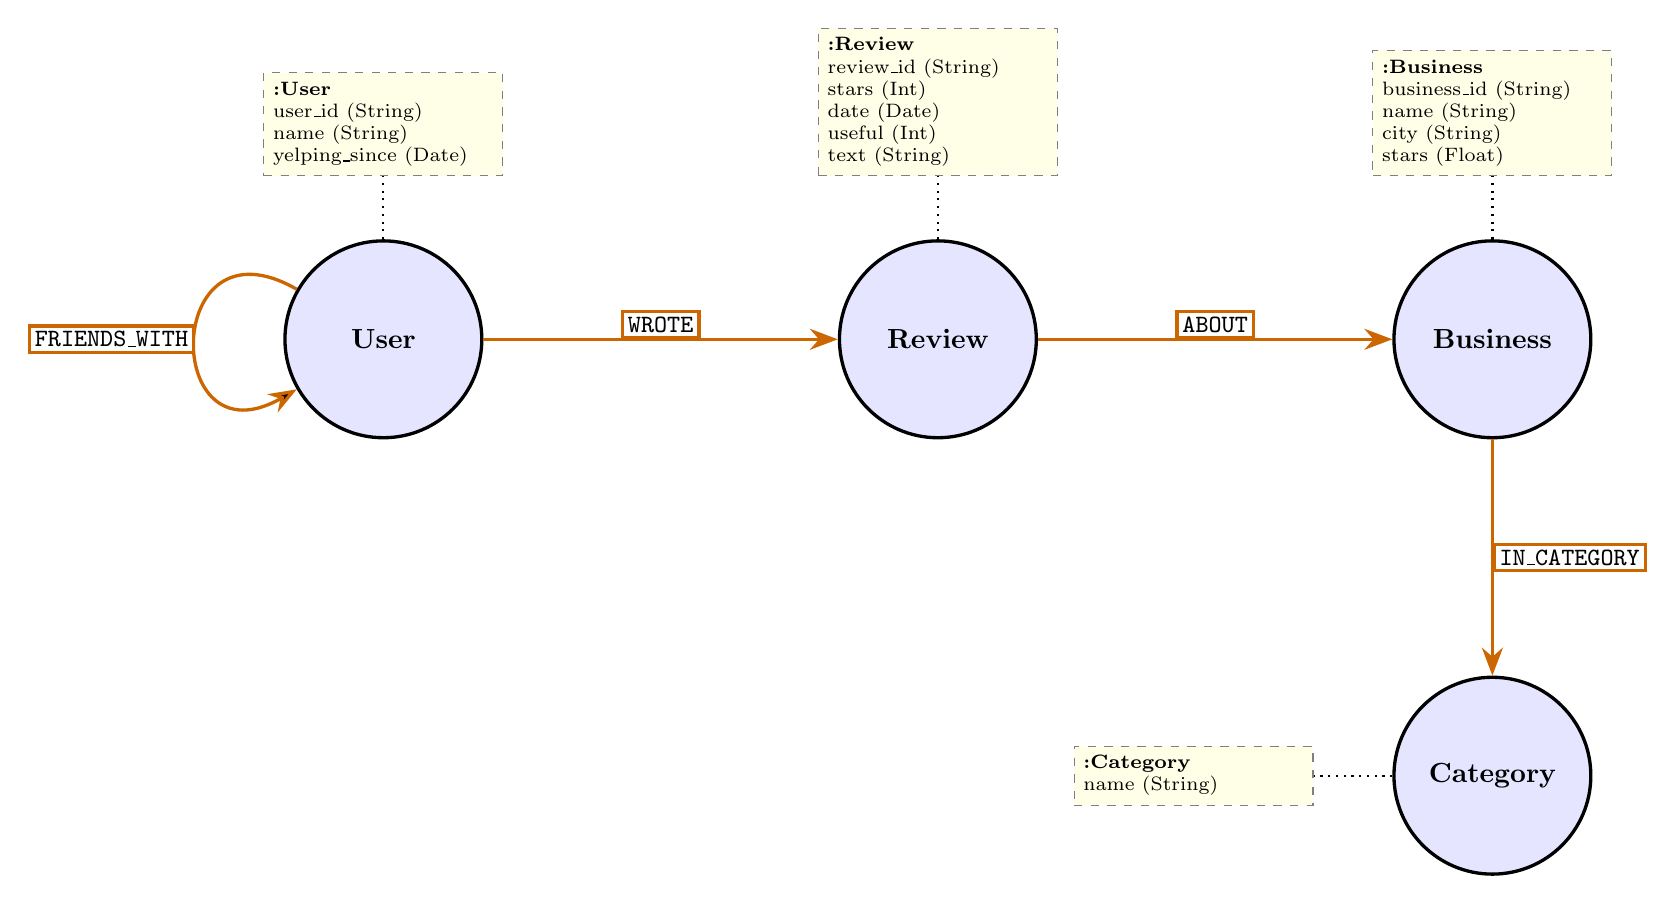
\begin{tikzpicture}[
    node distance=3.5cm and 4.5cm,
    % Nodes
    entity/.style={circle, draw=black, very thick, fill=blue!10, minimum size=2.5cm, align=center, font=\bfseries},
    % Relationships
    rel/.style={-{Stealth[scale=1.2]}, very thick, draw=orange!80!black},
    rel_label/.style={rectangle, fill=white, draw=orange!80!black, font=\small\ttfamily, inner sep=2pt},
    % Properties
    prop/.style={rectangle, draw=black!50, dashed, fill=yellow!10, text width=2.8cm, font=\scriptsize, align=left}
]

% Nodes
\node[entity] (user) {User};
\node[entity, right=of user] (review) {Review};
\node[entity, right=of review] (business) {Business};
\node[entity, below=3cm of business] (category) {Category};

% Self-relationship for User (Friends)
\path[rel] (user) edge [loop left, out=150, in=210, looseness=4] node[rel_label] {FRIENDS\_WITH} (user);

% Relationships connecting Nodes
\draw[rel] (user) -- node[rel_label, above] {WROTE} (review);
\draw[rel] (review) -- node[rel_label, above] {ABOUT} (business);
\draw[rel] (business) -- node[rel_label, right] {IN\_CATEGORY} (category);

% Properties (User)
\node[prop, above=0.8cm of user] (p_user) {
    \textbf{:User}\\
    user\_id (String)\\
    name (String)\\
    yelping\_since (Date)
};
\draw[dotted, thick] (user) -- (p_user);

% Properties (Review)
\node[prop, above=0.8cm of review] (p_review) {
    \textbf{:Review}\\
    review\_id (String)\\
    stars (Int)\\
    date (Date)\\
    useful (Int)\\
    text (String)
};
\draw[dotted, thick] (review) -- (p_review);

% Properties (Business)
\node[prop, above=0.8cm of business] (p_business) {
    \textbf{:Business}\\
    business\_id (String)\\
    name (String)\\
    city (String)\\
    stars (Float)
};
\draw[dotted, thick] (business) -- (p_business);

% Properties (Category)
\node[prop, left=1cm of category] (p_category) {
    \textbf{:Category}\\
    name (String)
};
\draw[dotted, thick] (category) -- (p_category);

\end{tikzpicture}
\end{document}
